
\section{Simulación del proceso evolutivo}
La simulación del proceso evolutivo es el encargado de simular los efectos de las variaciones
climáticas y el entorno en el ciclo de vida del Aedes aegypti.

El simulador del proceso evolutivo, es considerado como un proceso iterativo que inicia tomando
como parámetros de entrada la población inicial, y los datos climatológicos correspondientes al
periodo de simulación seleccionado. La población inicial es obtenida mediante la cantidad de
larvas observadas en los puntos de control que corresponden a la muestra utilizada para el estudio.
Por cada larva observada, en un punto de control ubicado en las coordenadas geográficas, $(x, y)$,
se inicializa un individuo con las mismas coordenadas del punto de control de origen.

\begin{figure}[!t]
    \centering
    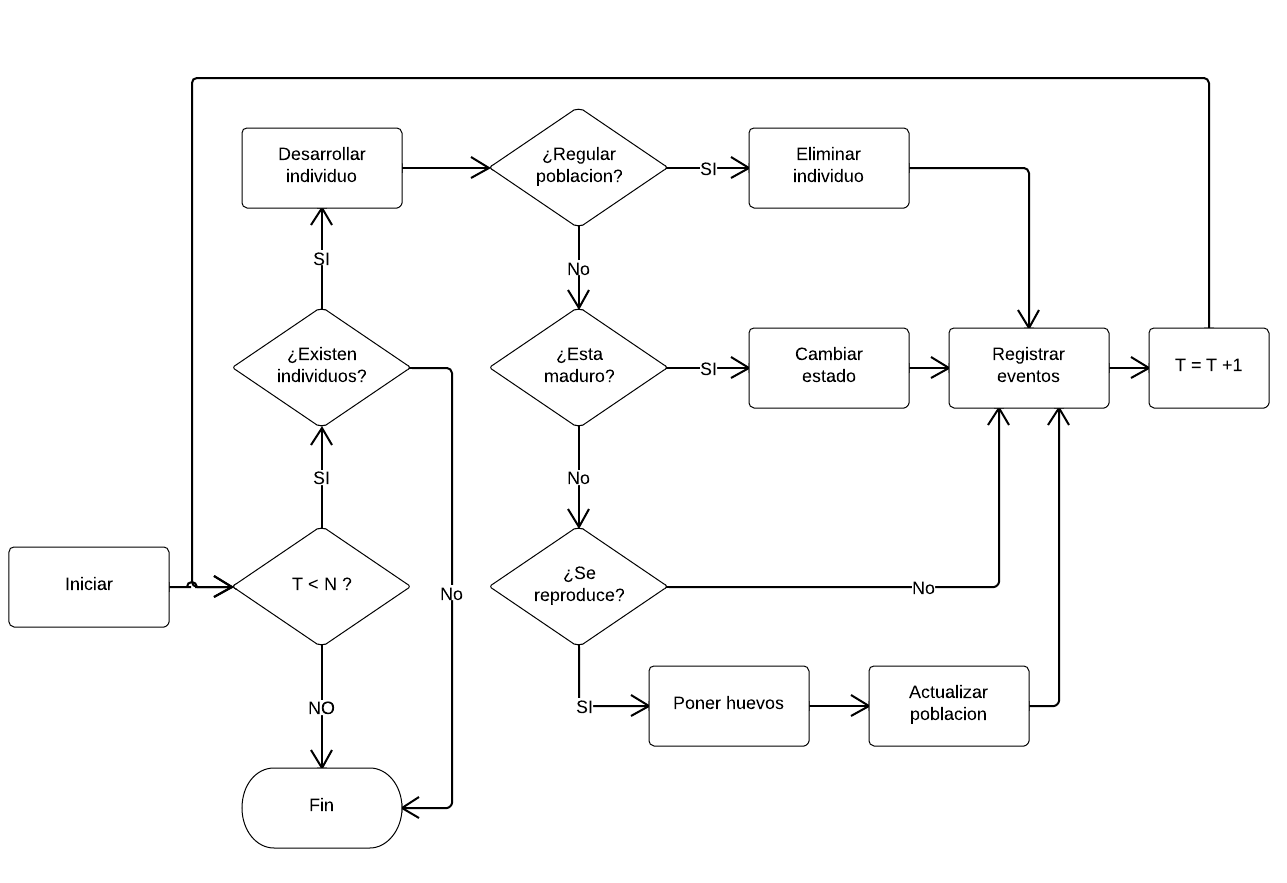
\includegraphics[width=0.45\textwidth]{../book/capitulo-5/graphics/algoritmo-evolutivo.png}
    \caption{\label{fig:algoritmo-evolutivo}Algoritmo del simulador del proceso evolutivo.}
\end{figure}

En la \figref{fig:algoritmo-evolutivo} se presenta el algoritmo del proceso evolutivo, donde el
periodo de simulación se encuentra representado por $T$.  El desarrollo de los individuos se
encarga de calcular las tasas de desarrollo correspondientes para cada etapa de su ciclo de vida,
con el fin de estimar su desarrollo considerando las condiciones climáticas. El cambio de estado
es consecuencia de la finalización de la etapa de desarrollo del individuo, donde el individuo ya
está listo para pasar a la siguiente etapa de su ciclo de desarrollo.

La regulación de la población es la encargada de calcular las tasas de mortalidad diaria,
correspondientes a cada etapa del ciclo de desarrollo del individuo, con el fin de reducir el
tamaño de la población debido a la mortalidad diaria de los individuos.

Si el individuo en cuestión corresponde a una hembra adulta inseminada, entonces esta se encuentra
en fase reproductiva. La postura de huevos se realiza respetando la tasa de desarrollo del ciclo
gonotrófico de las hembras. Si la hembra adulta ovipone, los huevos son añadidos a la población
como individuos en un estado inicial de \textit{HUEVO}.
